%%%% IACR Transactions TEMPLATE %%%%
% This file shows how to use the iacrtrans class to write a paper.
% Written by Gaetan Leurent gaetan.leurent@inria.fr (2020)
% Public Domain (CC0)


%%%% 1. DOCUMENTCLASS %%%%
\documentclass[journal=tches,submission]{iacrtrans}
%%%% NOTES:
% - Change "journal=tosc" to "journal=tches" if needed
% - Change "submission" to "final" for final version
% - Add "spthm" for LNCS-like theorems


%%%% 2. PACKAGES %%%%
\usepackage{lipsum} % Example package -- can be removed
\usepackage{graphicx}
\usepackage{listings}
\usepackage{booktabs} % provides \toprule / \midrule / \bottomrule
\usepackage{todonotes}
\usepackage[utf8]{inputenc}
\usepackage[T1]{fontenc}
\usepackage{amsmath, amssymb}
\usepackage{booktabs}
\usepackage{array}
\usepackage{tabularx} % provides the auto-wrapping X column
\usepackage{xcolor}
\usepackage{pifont}
% NOTE: do NOT load geometry here -- iacrtrans.cls already loads it with the
% journal's required page layout, and reloading it causes an option clash.
\usepackage{hyperref}

\newcommand{\runhead}[1]{\par\textbf{#1}\quad}
\newcommand{\code}[1]{\texttt{#1}}
\newcommand{\uaddr}[1]{\texttt{0x#1}}
\newcommand{\cmark}{\ding{51}}
\newcommand{\xmark}{\ding{55}}

\definecolor{darkviolet}{HTML}{9400D3}
\newcommand{\yvali}[1]{\todo[inline,color=darkviolet]{\textcolor{white}{\textbf{Yuval:} #1}}}
\newcommand{\yval}[1]{\todo[color=darkviolet,size=\footnotesize]{\textcolor{white}{\textbf{Yuval:} #1}}}

\definecolor{pink}{HTML}{f84f6c}
\newcommand{\sabrinai}[1]{\todo[inline,color=pink]{\textcolor{black}{\textbf{Sabrina:} #1}}}
\newcommand{\sabrina}[1]{\todo[color=pink,size=\footnotesize]{\textcolor{black}{\textbf{Sabrina:} #1}}}


\lstset{
  basicstyle=\ttfamily\footnotesize,
  breaklines=true,
  columns=fullflexible,
  keepspaces=true,
  frame=single,
  framesep=4pt,
  xleftmargin=2pt,
}

% Float placement: the defaults refuse a top float taller than 0.7\textheight
% and reserve 0.2\textheight for text, which pushed several tables one page past
% their discussion and deferred the tall figure to the end of the document.
\renewcommand{\topfraction}{0.9}
\renewcommand{\bottomfraction}{0.8}
\renewcommand{\textfraction}{0.08}
\renewcommand{\floatpagefraction}{0.75}
\setcounter{topnumber}{3}
\setcounter{bottomnumber}{2}
\setcounter{totalnumber}{4}

% The class passes "twoside" to article, which turns on \flushbottom.  On a page
% whose only stretchable glue is the "3.25ex plus 1ex" before-skip of the run-in
% \paragraph headings (Section 3), TeX inflates those skips to fill the page and
% they read as blank lines.  Let short pages end short instead, and use a smaller
% heading skip.  \SS@parafont keeps sectsty's bf+sf heading font.
\raggedbottom
\makeatletter
\renewcommand\paragraph{\@startsection{paragraph}{4}{\z@}%
      {1.75ex \@plus .3ex \@minus .2ex}%
      {-1em}%
      {\normalfont\normalsize\bfseries\SS@parafont}}
\makeatother

% iacrtrans loads hyperref via \AtEndPreamble; cleveref must come after it,
% so defer cleveref into the same hook.
\AtEndPreamble{%
  \usepackage[capitalize,nameinlink,noabbrev]{cleveref}% provides \cref / \Cref
  \crefname{lstlisting}{Listing}{Listings}%
  \Crefname{lstlisting}{Listing}{Listings}%
}

%%%% 3. AUTHOR, INSTITUTE %%%%
\author{Jane Doe\inst{1,2} \and John Doe\inst{1}}
\institute{
  Institute A, City, Country, \email{jane@institute}
  \and
  Institute B, City, Country, \email{john@institute}
}
%%%% NOTES:
% - We need a city name for indexation purpose, even if it is redundant
%   (eg: University of Atlantis, Atlantis, Atlantis)
% - \inst{} can be omitted if there is a single institute,
%   or exactly one institute per author


%%%% 4. TITLE %%%%
\title{MicroOpt: Microcode to Measurable Speed-ups}
%%%% NOTES:
% - If the title is too long, or includes special macro, please
%   provide a "running title" as optional argument: \title[Short]{Long}
% - You can provide an optional subtitle with \subtitle.

\begin{document}

\maketitle


%%%% 5. KEYWORDS %%%%
\keywords{Microcode \and Keccak \and Curve25519 \and Implementation}


%%%% 6. ABSTRACT %%%%
\begin{abstract}
  
\end{abstract}


%%%% 7. PAPER CONTENT %%%%
\section{Introduction}

Motivated by the need to better understand processors, many works present a detailed view into the microcode layer on x86 CPUs.
We now understand that it is a layer of abstraction used to implement the x86 instruction set. 
It allows complex intructions to be built over simpler ones and is also used to debug and patch the CPU after it has been manufactured.
The features that enable CPU designers to debug the CPU, have also been shown to be useful for other purposes, such as security and custom instructions.

High performance cryptographic software is closely shaped by the instruction set of the processor on which it runs. 
Implementations choose representations, instruction sequences, register allocations, and algorithmic variants according to the operations exposed by the architecture. 
On x86, this optimization normally ends at the architectural interface. 
The instructions themselves may be implemented by a lower level microcode, but software cannot ordinarily program that domain directly.

Microcode sits below that boundary. 
It implements part of the behavior exposed by the processor, but its execution environment is normally hidden from software. 
As a result, cryptographic implementation work rarely asks whether the microcode layer itself provides a useful computational substrate. 
The distinction matters because the interface available inside the processor need not match the one exposed through x86. 
If cryptographic computations can make effective use of this lower level interface, then the architectural instruction set is not necessarily the only relevant target for software optimization.

This paper studies that question experimentally. 
We investigate whether programmable x86 microcode can be used to execute performance critical cryptographic computation efficiently. 
Our goal is not to reproduce existing x86 implementations at a lower level. 
We instead ask whether the different execution model exposed by microcode changes how a cryptographic implementation should be organized, and whether those differences can translate into measurable performance advantages.

Cryptography offers a strong setting in which to study this question.
High performance implementations already receive extensive optimization at the architectural level. 
Competing against them therefore sets a stronger bar than demonstrating that computation can simply be moved into microcode. 
A useful microcode implementation must expose an advantage that survives comparison with carefully optimized native code. 
At the same time, cryptographic kernels contain structured computation with well understood costs, which allows us to identify where performnace might come from rather than treating the microcode domain as a black box.

We study this question through two case studies with different computational structure. 
Keccak $f[1600]$ is dominated by bitwise operationsand movement of a large internal state. 
Curve25519 is dominated by finite field arithmetic. 
Together they let us examine whether the microcode execution environment is useful across two different forms of cryptographic primitives. 
In each case, we begin from the operations required by the primitive and design the implementation around the capabilities and constraints of the microcode domain rather than around an existing x86 instruction sequence.
The motivations of this paper can be summarised as follows.

The resulting implementations show that programmable microcode can provide a performance advantage for cryptographic computation. 
Our Keccak implementation outperforms the optimized native implementations in our comparison, demonstrating that moving computation below the architectural interface can improve performance even against highly tuned x86 code. 
The Curve25519 case study reaches the same question through a different computational workload and shows how the microcode execution model can support an implementation that is organized differently from native x86 code. 

These results make the microcode layer relevant as more than an implementation detail of the processor. 
They show that mechanisms hidden below the architectural interface can be used to improve the performance of real cryptographic workloads. 
At the same time, the implementations reveal which properties of the microcode engine make those improvements possible and which constraints limit them. 
The broader result is therefore both practical and architectural. 
Programmable microcode can improve cryptographic performance, and studying why it does so exposes opportunities that are not visible from the architectural instruction set alone.

Our work makes the following contributions.

\begin{itemize}

\item We investigate programmable x86 microcode as an execution environment for performance critical cryptographic computation and develop a methodology for mapping cryptographic operations to that environment.

\item We implement Keccak $f[1600]$ in Goldmont microcode and show that the resulting implementation outperforms the optimized native implementations in our comparison.

\item We implement the performance critical arithmetic of X25519 in microcode and show that the microcode execution model permits arithmetic dependencies to be organized differently from ordinary x86 code.

\item We use controlled ablation experiments to identify which microcode capabilities account for the observed performance and which constraints limit their use.

\end{itemize}

Together, these case studies show that programmable microcode is not merely another way to encode an existing instruction sequence. 
It exposes a different execution interface, and that interface can change both the organization and the performance of cryptographic computation.

%\yvali{Start each sentence in a new line. If you break a sentence into multiple lines, try to choose break points that agree with the sentence structure.}

\section{Background and Programming Model}
\label{sec:background}

%\yvali{Can you add a figure that shows the process of generating microcode, including patch mechanism?  Something that shows instructions arriving from top, microops emitted from bottom, and shows the fast and slow pathes, as well as the patch mechnism?} 

%\yvali{We need to discuss somewhere that short sections of code do not provide benefit, so we aim at larger pieces.}

\section{Methodology}
\label{sec:methodology}

In this section we describe the methodology used throughout the following case studies.
We explain how we identify performance critical cryptographic computation and map it to Goldmont microcode.
We then describe how the constraints of the microcode engine guide the implementation and how we validate correctness and measure performance.

\begin{figure}[t]
    \centering
    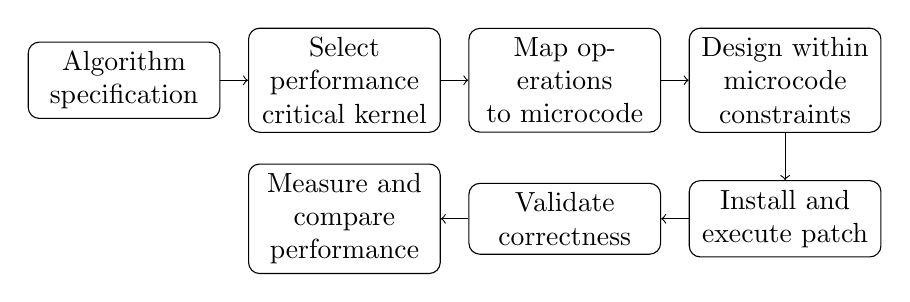
\begin{tikzpicture}[
        node distance=0.35cm,
        every node/.style={
            draw,
            rounded corners,
            align=center,
            minimum height=0.75cm,
            text width=2.2cm
        }
    ]

    \node (spec) {Algorithm\\specification};
    \node[right=of spec] (select) {Select performance\\critical kernel};
    \node[right=of select] (map) {Map operations\\to microcode};
    \node[right=of map] (design) {Design within\\microcode constraints};

    \node[below=0.6cm of design] (impl) {Install and\\execute patch};
    \node[left=of impl] (validate) {Validate\\correctness};
    \node[left=of validate] (measure) {Measure and\\compare performance};

    \draw[->] (spec) -- (select);
    \draw[->] (select) -- (map);
    \draw[->] (map) -- (design);
    \draw[->] (design) -- (impl);
    \draw[->] (impl) -- (validate);
    \draw[->] (validate) -- (measure);

    \end{tikzpicture}

    \caption{Methodology used to develop and evaluate the microcode implementations.}
    \label{fig:methodology}
\end{figure}

\paragraph{Kernel selection.}
We begin from the specification of each algorithm and identify the computation that dominates its execution cost.
The selected kernel is expressed in terms of the operations required by the algorithm rather than the x86 instructions used by an existing implementation.
This keeps the design independent of an existing instruction mapping and allows the implementation to use capabilities exposed directly by the microcode engine.

\paragraph{Microcode design.}
We map the selected computation to the micro-operations available on Goldmont.
Internal temporary registers provide additional storage and some micro-operations expose functionality without a direct x86 equivalent.
Control flow can also remain inside the microsequencer without returning to ordinary x86 code.

The design must fit within the resources provided by the microcode engine.
Goldmont provides 128 triads of patch capacity and 16 temporary registers.
These constraints determine which values remain resident and which values must be moved or recomputed.
They also determine whether loops remain inside the microsequencer.
When several mappings are possible we favor fewer executed micro-operations and less data movement.

During the design phase we established several undocumented characteristics of Goldmont microcode experimentally.
These include triad hazard semantics and memory operation limits as well as addressing restrictions and the construction of control flow inside the microsequencer.
Each implementation must therefore satisfy both the architectural constraints of the algorithm and the execution constraints that we identified for the microcode engine.

\paragraph{Patch organization.}
The completed routine is installed as a microcode patch in the Microcode RAM (MSRAM).
A match register redirects execution from an existing MSROM entry point to code placed in MSRAM.
Figure~\ref{fig:decodeandpatch} shows this mechanism in the Goldmont decode path.

Each transition from MSROM to MSRAM costs around 7 cycles.
We therefore place larger computational kernels behind each redirection rather than dividing the implementation across many small patches.
This amortizes the fixed redirection cost over more useful computation.
Patch capacity of 128 triads places an upper limit on this granularity and the resulting design tries to balance these two constraints.

The surrounding native program invokes the patched instruction when the cryptographic routine is required.
No processor hardware is modified.
The implementation instead uses execution resources already present in the Goldmont core.

\paragraph{Validation and evaluation.}
We validate functional correctness before evaluating performance.
Each microcode implementation is tested against an established implementation of the same algorithm.
Identical inputs must produce the corresponding reference result.

Performance is measured using cycle counts on the same Goldmont system used for the native implementations.
The evaluation includes optimized implementations for the same x86 platform.
Repeated measurements characterize execution cost and the median provides the primary comparison.
%We use ablation experiments where appropriate to isolate design choices that contribute directly to the final result.
%Each ablation removes one technique while leaving the remainder of the implementation unchanged.

The two case studies exercise different properties of the microcode engine.
Keccak places pressure on register capacity and relies primarily on bitwise operations and rotations.
Curve25519 instead relies on multi precision field arithmetic and repeated carry propagation.
Together they allow us to apply the same methodology to two different forms of cryptographic computation.
\begin{figure}[tbp]
  \centering
  \includegraphics[width=0.9\linewidth]{DecoderAndPatch.png}
  \caption{Decode path on Goldmont and the effect of a microcode patch.
  Macroinstructions decoded by the microsequencer have their MSROM address checked against the match registers.
  An unmatched address (\code{rdrand}) is served from the microcode ROM, while a matched address (\code{cpuid}, redirected to \uaddr{74dc}) is served from the microcode RAM, so that our custom triads are emitted in place of the original ones.}
  \label{fig:decodeandpatch}
\end{figure}
\section{Case Study 1: Keccak-f[1600] in Microcode}
\label{sec:keccak}

%\yvali{Restructure this (and the next) section.  You want four main parts, each typically one but maybe more sub sections:\\
%$\bullet$~\textbf{Challenges:} What current implementations do, what their limitations are.\\
%$\bullet$~\textbf{Strategy} the general implementation strategy.  Benefit from large code, more registers, and tight loop in microcode.  Perform the full 24 rounds. Etc.\\
%$\bullet$~\textbf{Implementation:} Any non-trivial thing in the implementation, also, some statistics on, e.g., how many triads we use.\\
%$\bullet$~\textbf{Evaluation:} How well does it perform?

%%%%\yval{Why do we care about field arithmetic here?}
%\yval{What are in-place looping and indexed addressing? Why are they relevant?}
%\yval{This is not the time to talk about this level of contribution.  You first need to describe the implementation, then evaluate it, then maybe toot your horn.}

\subsection{Challenge and Prior Techniques}
\label{sec:keccak-challenge}

Optimized implementations of Keccak are shaped by three architectural properties.
These are the number of available registers, the instructions provided for rotating and combining 64-bit values, and the cost of moving the 25-lane state between registers and memory.
Each lane contains 64 bits, so the complete Keccak-$f[1600]$ state occupies 1600 bits.
A processor that cannot hold this state and the intermediate values of a round in registers must repeatedly store lanes to memory and load them again when they are needed.
Even when these accesses are quick, they consume instructions, load and store resources, and registers needed for address calculation.

The eXtended Keccak Code Package, or XKCP, contains implementations adapted to different processor architectures~\cite{XKCP}.
These implementations combine several established optimization techniques, including lane complementing, plane-by-plane processing, round unrolling, and SIMD parallelism.
Each technique addresses a different architectural limitation.
Lane complementing reduces the number of Boolean operations required by the nonlinear step.
Plane-by-plane processing limits the amount of state that must be active at one time and reduces unnecessary transfers between temporary arrays.
Round unrolling removes loop-control instructions and allows the register assignment of one round to be incorporated into the following round.
SIMD implementations use vector registers either to manipulate several lanes together or to evaluate several independent permutations in parallel.

Scalar x86-64 nevertheless imposes a fundamental register-capacity constraint.
The architecture exposes 16 general-purpose registers, and some of them are required for the stack pointer, addresses, loop control, and temporary values.
The 25 lanes of Keccak therefore cannot all occupy architectural registers simultaneously.
Optimized implementations can choose which lanes to keep resident, arrange loads early enough to hide part of their latency, and delay stores until registers must be reused.
These techniques reduce the cost of spilling, but they do not remove its underlying cause.
Some portion of the state must still move through memory because the architectural register file is smaller than the state itself.
The microcode environment changes this constraint.
In addition to the architectural registers, a microcode patch can use 16 temporary registers named \code{TMP0} through \code{TMP15}.
These registers remain available while the patch is executing and are not visible to ordinary x86 software.


\Cref{tab:methods} summarizes how established techniques map to the Goldmont microcode model.
Some techniques remain useful, while others solve problems that are irrelevant in this environment.

\begin{table}[htbp]
\centering
\small
\begin{tabular}{@{}p{0.25\linewidth}p{0.39\linewidth}c@{}}
\toprule
Technique & Relevance to Goldmont microcode & Used \\
\midrule
Lane Complementing & Native \code{NOTAND} already implements the nonlinear term & \xmark \\
Lazy Rotations & Constant-time immediate 64-bit rotate is available & \xmark \\
Bit Interleaving & Native 64-bit registers and operations are available & \xmark \\
In-place processing & Avoids a second 25-lane state & \cmark \\
Whole-state residency & The combined architectural and temporary register file holds all lanes & \cmark \\
Native \code{NOTAND} & Reduces each $\chi$ output to two $\mu$ops & \cmark \\
\bottomrule
\end{tabular}
\caption{Applicability of established Keccak implementation techniques to the Goldmont microcode model.}
\label{tab:methods}
\end{table}

Lane Complementing changes the representation of selected lanes so that parts of $\chi$ can be evaluated with fewer explicit bitwise negations.
This is valuable when the processor must compute the expression $(\lnot B[x+1,y])\land B[x+2,y]$ using separate NOT and AND instructions.
Microcode instead provides the operation \code{NOTAND}, which computes this complete expression in one $\mu$op.
Lane complementing is therefore not used.

Lazy Rotation is useful when 64-bit rotations are expensive.
It tracks each lane's logical rotation and incorporates it into later operations, reducing explicit rotations at the cost of a more complex state representation.
Microcode provides \code{ROL\_DSZ64\_DRI}, which rotates a 64-bit value by a constant amount in one $\mu$op.
All Keccak rotation offsets are known statically, so the direct rotation already has the desired form.
Lazy Rotation would increase implementation complexity without decreasing the operation count.

Bit Interleaving addresses processors that lack native 64-bit operations.
It represents one 64-bit lane using two smaller words, with one word holding the even-positioned bits and the other holding the odd-positioned bits.
A 64-bit rotation can then be expressed using operations on the two smaller words.
This representation is useful on 16-bit or 32-bit processors, but it doubles the number of registers required for each lane and introduces conversion overhead at permutation boundaries.
Microcode supports native 64-bit registers, XORs, Boolean operations, and rotations, so bit interleaving would consume additional registers without providing an arithmetic advantage.

In-place processing remains directly relevant.
A textbook description of a Keccak round commonly uses a second 25-lane array to hold the output of $\rho$ and $\pi$ before $\chi$ is evaluated.
Materializing this array would defeat the purpose of keeping the state resident because it would require either another 25 registers or repeated memory transfers.
Our implementation instead transforms the state within its existing registers.
During the $\chi$ step, all five temporary values for a row are computed before that row is updated.
This lets us update the state in place without using a second state array.

The enlarged register file therefore enables a stronger optimization than merely reducing the number of spills.
It removes state-lane spills from the round body entirely.
The 25 lanes are transferred between memory and registers only at the beginning and end of the permutation.
During all 24 rounds, the state remains in registers and is updated in place.

\subsection{Strategy}
\label{sec:keccak-design}

Our strategy is to make one hooked macroinstruction perform the complete permutation.
Before the first round begins, the implementation saves \code{RSP} and loads the 25 state lanes into 13 architectural registers and 12 temporary registers.
The patch then executes the same round body 24 times.
After each round, a sequence-word branch returns to the beginning of the round body until all round constants have been consumed.
\sabrina{Reconsider what follows. DO we need this here?}
Within each round, the five $C$ parities are spilled to a centered scratch buffer, while the more frequently used $D$ values remain in registers.
The application of $\theta$, together with $\rho$ and $\pi$, is fused into a single in-place traversal.
After $\chi$ and $\iota$, a same-triad compare-and-branch operation returns execution to the beginning of the round until all 24 round constants have been consumed.
Once the final round is complete, the implementation stores the 25 state lanes back to memory and restores \code{RSP}.

This organization loads each of the 25 Keccak lanes from memory once at the beginning of the permutation and stores each lane back once after the final round.
Memory traffic during each round is limited to five stores and ten loads for the parity values, two loads used to obtain the round constant, and one store for the round counter.
The main implementation challenges are assigning all simultaneously needed values to the available registers, ensuring that every lane is in its expected register when the next round begins, and fitting the complete microcode routine into the space available in MSRAM.


\subsection{Implementation}

\subsubsection{Whole-state Residency and Register Budget}
\label{sec:residency}

The first technique we adopt is whole-state residency. %CITATION: Becker and Kannwischer's loopable AArch64 implementation
All twenty-five lanes remain in registers from their initial load at the beginning of the permutation until they are stored back to memory after the final round.
No lane is spilled while the permutation is being computed.
Table~\ref{tab:regmap} summarizes the register allocation.
Thirteen architectural registers hold lanes 0 through 12, while twelve temporary registers hold lanes 13 through 24, following the flat index $i = x + 5y$.

\begin{table}[htbp]
\centering
\small
\setlength{\tabcolsep}{5pt}
\begin{tabular}{@{}c|ccccc@{}}
\toprule
 & $x = 0$ & $x = 1$ & $x = 2$ & $x = 3$ & $x = 4$ \\
\midrule
$y = 0$ & \code{RDI} (0, $\rho$0)  & \code{RSI} (1, $\rho$1)   & \code{RBX} (2, $\rho$62)  & \code{RDX} (3, $\rho$28)  & \code{RBP} (4, $\rho$27) \\
$y = 1$ & \code{R8} (5, $\rho$36)  & \code{R9} (6, $\rho$44)   & \code{R10} (7, $\rho$6)   & \code{R11} (8, $\rho$55)  & \code{R12} (9, $\rho$20) \\
$y = 2$ & \code{R13} (10, $\rho$3) & \code{R14} (11, $\rho$10) & \code{R15} (12, $\rho$43) & \code{TMP0} (13, $\rho$25) & \code{TMP1} (14, $\rho$39) \\
$y = 3$ & \code{TMP2} (15, $\rho$41) & \code{TMP3} (16, $\rho$45) & \code{TMP4} (17, $\rho$15) & \code{TMP5} (18, $\rho$21) & \code{TMP6} (19, $\rho$8) \\
$y = 4$ & \code{TMP7} (20, $\rho$18) & \code{TMP8} (21, $\rho$2) & \code{TMP9} (22, $\rho$61) & \code{TMP10} (23, $\rho$56) & \code{TMP11} (24, $\rho$14) \\
\bottomrule
\end{tabular}

\vspace{4pt}
\begin{tabularx}{\linewidth}{@{}lX@{}}
\toprule
\code{RAX}, \code{TMP12}--\code{TMP15}
& hold $D[0],\ldots,D[4]$ during $\theta$ and are reused for temporary values during $\chi$ \\
\code{RCX}
& holds the fixed base address of the working buffer throughout the permutation \\
\code{RSP}
& is saved to memory, used as temporary workspace during $\theta$ and $\pi$, and restored before returning \\
\bottomrule
\end{tabularx}
\caption{Register allocation for the $5\times5$ Keccak state and the auxiliary values required during each round. For each of the 25 lanes, the table lists the assigned register, the flat index $i=x+5y$, and the corresponding $\rho$ rotation offset. The mapping uses all 16 architectural registers and all 16 temporary registers available to the microcode patch.}
\label{tab:regmap}
\end{table}

A register allocation that reserves the stack pointer provides only 31 usable registers and therefore we fall one register short.
Twenty-five registers hold the Keccak state, five hold the $\theta$ mixing values $D[0],\ldots,D[4]$, and one holds the base address of the working buffer.
One additional register is required as the second accumulator in the balanced parity computation described in \Cref{sec:paritytree} and as temporary storage during the in-place cycle traversal described in \Cref{sec:cyclewalk}.

We obtain this additional register by temporarily repurposing \code{RSP}.
The patch does not access the stack while \code{RSP} is being used for intermediate values, and its original value is restored before execution returns from the hooked macroinstruction.
%Our \code{probe\_rsp} test confirmed that \code{RSP} can be saved in a dedicated slot of the working buffer before the state is loaded and restored after the final state values have been written to memory without disrupting subsequent x86 execution.
%This requires one additional store and one additional load per permutation.

The register budget also requires us to choose which $\theta$ intermediates remain in registers. 
We retain $D$ and spill $C$ because $D$ has more uses during each round. 
Each parity $C[x]$ is read twice, once as $C[x-1]$ and once as $C[x+1]$, giving ten reads across all five parities. 
By contrast, each $D[x]$ is applied to the five lanes in its column, giving 25 reads across all five mixing values. 
Spilling $C$ therefore requires five stores and ten loads, whereas spilling $D$ would require 25 loads. 
Retaining $D$ reduces the resulting memory traffic by ten operations per round.

The traversal order induced by $\pi$ further favors retaining $D$ in registers. 
The cycle walk interleaves lanes from different columns, so the five uses of a given $D[x]$ are distributed across the traversal. 
If we spilled $D$, we would therefore need to reload the corresponding value for each lane rather than amortize one load across the entire column. 
We instead spill the five $C[x]$ values to a nearby scratch region and reload them when computing $D$. 
The proximity of this region supports store-to-load forwarding. 
We then retain all five $D[x]$ values in registers throughout the cycle walk. 
This storage strategy adapts $\theta$ to Goldmont’s register constraints without changing the Keccak transformation itself.


\subsubsection{A microcode-resident round loop}
\label{sec:loop}

We execute all 24 rounds within the microsequencer. 
If our implementation returned to ordinary x86 code after each round, it would lose the twelve state lanes held in the internal temporary registers. 
We also cannot fully unroll the permutation within the patch. 
Replicating the 56-triad round body 24 times would require 1344 triads, which exceeds the 128-triad capacity. 
We therefore retain control in microcode and repeatedly execute a single round body.

We use the position in the round-constant table as the loop variable. 
Using a round-constant pointer to control a Keccak loop is established practice. 
Our implementation adapts this approach to the control-flow mechanisms available in Goldmont microcode.
%  CITATION: cite the OpenSSL x86-64 Keccak loop here.

At the end of each round, our implementation executes the three triads shown in Listing~\ref{lst:roundloop}. 
The first triad loads the current round constant. 
The second applies the constant to lane 0, advances the table position by eight bytes, and stores the updated position. 
In the final triad, we XOR the updated position with the terminal offset of 320. 
The result becomes zero only after the final round and sets \code{ZF} accordingly.

Our experiments showed that \code{UJMPCC} evaluates \code{ZF} rather than the register operand encoded in the instruction. 
When the XOR result is nonzero, the branch returns to \uaddr{7c68}, which contains the first triad of the round body. 
When the result is zero, execution leaves the loop. 
We place the XOR and \code{UJMPCC} in the same triad to ensure that the branch observes the flag produced by the comparison.

\begin{lstlisting}[caption={The three triads that close each Keccak round. Our implementation applies $\iota$, advances the round-constant position, and returns to the beginning of the round body until it consumes the final constant.},label={lst:roundloop}]
{ LDZX_DSZ64_ASZ32_SC1_DRR(TMP13, RCX, TMP14, SEG_DS), NOP, NOP, NOP_SEQWORD },
{ XOR_DSZ64_DRR(RDI, RDI, TMP13), ADD_DSZ64_DRI(TMP14, TMP14, 8),
STAD_DSZ64_ASZ32_SC1_RRI(TMP14, RCX, 112, SEG_DS), NOP_SEQWORD },
{ XOR_DSZ64_DRI(TMP12, TMP14, 320), NOP,
UJMPCC_DIRECT_NOTTAKEN_CONDNZ_RI(TMP12, 0x7c68), NOP_SEQWORD },
\end{lstlisting}

Because we reuse the same round body, every lane must occupy the same register whenever execution returns to the loop entry. 
This constraint separates this work from every fully unrolled register-resident implementation. 
A fully unrolled implementation can absorb $\pi$ into the register names used by the following round because each round has a distinct instruction sequence. 
Our implementation re-enters the same sequence, so we must restore the register assignment during every round. 
We perform this register transport using the cycle walk described next.

\subsubsection{Fused cycle-walk transport for the $\theta$ apply, $\rho$ and $\pi$}
\label{sec:cyclewalk}

The conventional formulation of a Keccak round writes an intermediate array $B$. 
For each lane, it applies $\theta$ by XORing the lane with the corresponding $D$ value, applies the $\rho$ rotation, and writes the result to the destination specified by $\pi$. 
We avoid this intermediate array by following the established in-place approach based on the cycle structure of $\pi$.

As a permutation of the 25 lane positions, $\pi$ consists of a fixed point at lane 0 and a single cycle containing the remaining 24 lanes. 
This cycle is
\[
(1\ 10\ 7\ 11\ 17\ 18\ 3\ 5\ 16\ 8\ 21\ 24\ 4\ 15\ 23\ 19\ 13\ 12\ 2\ 20\ 14\ 22\ 9\ 6).
\]
We traverse the cycle in reverse and preserve one value in a temporary register to break the cycle. 
This order ensures that we consume the previous contents of each destination register before overwriting them. 
The cycle decomposition and the use of one temporary are established Keccak implementation techniques.
%CITATION: standardized/reference 24-word cycle.
Our implementation extends this traversal by applying $\theta$ and $\rho$ during each register transfer. 
For every hop in the cycle, we execute
\[
\mathrm{REG}[\mathrm{dst}] \leftarrow
\mathrm{ROL}\bigl(\mathrm{REG}[\mathrm{src}] \oplus
D[\mathrm{col}(\mathrm{src})],\rho[\mathrm{src}]\bigr).
\]
The algorithmic fusion of these operations with the $\pi$ traversal is also established. 
We adapt it to Goldmont by expressing the complete traversal as register-to-register micro-operations while restoring the fixed lane-to-register assignment required at the round-loop boundary.
%cite: Linux sha3_generic.c or an equivalent fused cycle walk.

We use the borrowed \code{RSP} register to break the 24-lane cycle. 
For each lane in the cycle, we execute one XOR and one rotation. 
These operations require no loads because we retain all five $D[x]$ values in registers. 
Lane 0 remains fixed under $\pi$ and has a $\rho$ offset of zero, so we apply only the corresponding XOR. 
The complete traversal therefore requires 25 XORs, 24 rotations, and one register copy.
In total, we implement the $\theta$ apply, $\rho$, and $\pi$ with 50 micro-operations, one temporary register, and no memory accesses.

Memory-resident implementations can apply the same cycle walk with one temporary word, but they must load and store each lane as it moves through the cycle. 
By retaining the complete state in registers, our implementation performs the same transport without a second state array and without transferring lanes through memory.

We pack two consecutive cycle hops into one triad by relying on the sequential semantics of its execution slots. 
In the following triad, slot 0 reads \code{R12}, slot 1 rotates the resulting value, and slot 2 overwrites \code{R12} with the value assigned to the next lane. 
This packing relies on a write-after-read dependency on \code{R12} within the triad.

\begin{lstlisting}
{ XOR_DSZ64_DRR(R9, R12, TMP15), // slot 0: R9 <- R12 xor TMP15
ROL_DSZ64_DRI(R9, R9, 20), // slot 1: R9 <- rol(R9, 20)
XOR_DSZ64_DRR(R12, TMP9, TMP13), // slot 2: R12 <- TMP9 xor TMP13
NOP_SEQWORD },
\end{lstlisting}

\paragraph{Reusing the $D$ registers during $\chi$.}
\label{sec:chireuse}

For each row, $\chi$ computes
\[
A[x,y]=B[x,y]\oplus((\lnot B[x+1,y])\wedge B[x+2,y]).
\]
To evaluate $\chi$ in place, we must preserve the original five lanes until we have computed all five nonlinear terms. 
Existing in-place implementations commonly use five temporary values for this purpose. 
Our register allocation provides these temporaries without requiring additional lane copies.

The five registers that hold $D[0],\ldots,D[4]$ become dead when we complete the fused traversal. 
We reuse these registers immediately as the five temporaries required by $\chi$. 
For each row, we first compute all five \code{NOTAND} results and store them in \code{RAX} and \code{TMP12}--\code{TMP15}. 
We then apply the five XORs to update the row in place. 
Our Goldmont-specific contribution is this exact reuse of the dead $D$ registers within the constrained allocation, rather than the general use of five temporaries for an in-place $\chi$ implementation.

We also exploit the Goldmont micro-operation \code{NOTAND\_DSZ64\_DRR}, which computes $(\lnot a)\wedge b$ in a single operation. 
Native x86 code on this processor cannot use \code{ANDN} because Goldmont does not implement BMI2. 
It must instead issue a \code{NOT} followed by an \code{AND}. 
Our implementation completes $\chi$ with 25 \code{NOTAND} operations and 25 XORs, which we pack into 17 triads.

\begin{lstlisting}
{ NOTAND(RAX, RSI, RBX), NOTAND(TMP12, RBX, RDX),
NOTAND(TMP13, RDX, RBP), NOP_SEQWORD },
{ NOTAND(TMP14, RBP, RDI), NOTAND(TMP15, RDI, RSI),
XOR(RDI, RDI, RAX), NOP_SEQWORD },
{ XOR(RSI, RSI, TMP12), XOR(RBX, RBX, TMP13),
XOR(RDX, RDX, TMP14), NOP_SEQWORD },
{ XOR(RBP, RBP, TMP15), NOTAND(RAX, R9, R10),
NOTAND(TMP12, R10, R11), NOP_SEQWORD },
\end{lstlisting}

\paragraph{Latency scheduling for $\theta$ and $\iota$.}
\label{sec:paritytree}

We compute each column parity $C[x]$ by reducing five lanes with XOR. 
A serial reduction requires four dependent XORs and therefore has a dependency depth of four. 
This computation lies at the beginning of the round’s critical path because all subsequent operations depend on $D$ and, in turn, on $C$.

This placement suggests shortening the chain, and the borrowed \code{RSP} provides a second accumulator with which to do so.
The resulting balanced expression
\[
C[x]=\bigl((A[x]\oplus A[x+5])\oplus(A[x+10]\oplus A[x+15])\bigr)
\oplus A[x+20]
\]
makes the first two XORs independent, so they occupy separate slots of the same triad, and reduces the dependency depth from four to three at an unchanged operation count and patch footprint.
We implemented this schedule and measured it, and it does not pay for itself: reinstating it costs 1.2\% against the serial reduction (\Cref{tab:results-ablation}).
The shipped kernel therefore performs the serial reduction.
Because the two forms have identical triad and operation counts, the difference is a scheduling effect rather than a difference in work.
The balanced form holds a second accumulator live across each column, and the parity chain was evidently not the binding constraint.
We report the measurement and do not claim a mechanism for it.

Our register allocation leaves no register available for a round constant. 
We therefore store the 24 constants in the working buffer and use the loop variable to hold the byte position of the current constant. 
The host initializes this position to $(32-16)\cdot8=128$, and our round body advances it by eight bytes after each round.

This representation allows us to load the current constant without first shifting or otherwise transforming a round counter. 
The $\iota$ step requires one load of the table position, one indexed load of the constant, and one XOR into lane 0. 
We update and store the table position only after fetching the constant, so these loop-control operations do not extend the dependency path of $\iota$.

\subsubsection{Patch layout and verification}

The complete patch occupies 108 triads: a 26-triad prologue, a 56-triad round body including loop control, and a 26-triad epilogue.
The prologue and epilogue each contain 25 state transfers plus one operation to save or restore \code{RSP}.
Although isolated triads containing two memory operations executed successfully in our probes, packing many such triads back to back caused hard faults.
The implementation therefore observes the conservative limit of one memory operation per triad.

Looping keeps the static image within the 128-triad patch RAM, but a complete permutation dynamically executes
\[
26 + 24\cdot56 + 26 = 1396
\]
triads and 3700 non-NOP $\mu$ops.
Branch targets are absolute patch RAM addresses, so the round loop target is fixed by the length of the prologue and lands immediately after it at \uaddr{7c68}.
The schedule admits no load-to-use dependence within a triad and places the final XOR comparison and \code{UJMPCC} in the same triad.

We validate the installed patch itself rather than a model of it.
The hardware harness executes the patch on 1000 random states and compares every lane with a direct 24-round reference.
It also checks the full published $f(0)$ and $f(f(0))$ states, the latter providing a nonzero-input known-answer test independent of the reference function.
Both known-answer tests are fixed published constants rather than values recomputed in process, so an error common to the reference and the patch cannot pass unnoticed.

\subsection{Performance Evaluation}

%\paragraph{Experimental setup.}
%All results come from the Intel Celeron N3350 with the Goldmont core described in \Cref{sec:measurement}. 
%Turbo remains disabled, the processor stays pinned to its base
%frequency, and a single process times every implementation.
%The native implementations build under the six GCC and Clang releases and four optimisation levels listed in \Cref{sec:measurement}.
%Each implementation then keeps the configuration that achieved the lowest median.

\paragraph{Constant time behaviour.}
The microcode kernel preserves the input independent control flow and addressing of Keccak $f[1600]$.
The patch contains 108 triads and one conditional operation, which tests the public round constant cursor.
The same cursor addresses the only indexed load.
Every state lane resolves through a fixed displacement, and every $\rho$ offset is fixed in the patch image.
No data dependent branch and data dependent address therefore arise during execution.
We assume that the underlying micro-operations have data independent latency, as constant time native implementations of Keccak do.

The comparison covers every executable member of the SUPERCOP \texttt{crypto\_hash/\allowbreak keccakc1024} family on this Intel core with 64 bit support.
The XKCP single permutation kernel and the OpenSSL scalar assembly for x86 64 join the same comparison.
Each contender computes the same primitive on the same core, and the timed region includes the dispatch or call required to invoke it.
\Cref{sec:measurement} describes the remaining asymmetry in that region. \Cref{tab:results-keccak} reports the results.

\begin{table}[htbp]
\centering
\caption{Performance comparison of Keccak $f[1600]$ permutations on the Goldmont N3350.
Each implementation appears in its best configuration across the 24 compiler and optimisation configurations.
All values are cycles per permutation, and the headline value is the median over 200 measurement batches.
Relative cost divides each native median by the microcode median.
A value above~1 indicates that the microcode kernel is faster. 
The microcode row reports the looped single firing kernel from \Cref{sec:keccak-design}.
\Cref{tab:res-keccak-dispersion} describes the method of each implementation and
reports its minimum and its interval between $p_{10}$ and $p_{90}$.}
\label{tab:results-keccak}
\footnotesize
\setlength{\tabcolsep}{4pt}
\begin{tabular}{@{}lrrl@{}}
\toprule
Implementation & Median & Rel. cost & Best config \\
\midrule
\textbf{microcode} & \textbf{1895} & \textbf{1.000$\times$} & GCC 11 O3 \\
\midrule
openssl/opt64lcu24            & 2054 & 1.084$\times$ & GCC 11 O3 \\
x86\_64\_asm      & 2073 & 1.094$\times$ & GCC 11 Os \\
xkcp\_g64lc       & 2160 & 1.140$\times$ & GCC 12 Os \\
opt64lcu6         & 2219 & 1.171$\times$ & Clang 17 O3 \\
xkcp\_g64         & 2274 & 1.200$\times$ & Clang 14 O2 \\
simple            & 2372 & 1.252$\times$ & GCC 11 O3 \\
opt64u6           & 2397 & 1.265$\times$ & GCC 11 O2 \\
sseu2             & 3055 & 1.612$\times$ & Clang 17 O2 \\
mmxu1             & 3955 & 2.087$\times$ & Clang 14 O3 \\
opt64lcu24shld    & 10069 & 5.313$\times$ & Clang 17 Os \\
x86\_64\_shld     & 10115 & 5.338$\times$ & Clang 18 O2 \\
\bottomrule
\end{tabular}
\end{table}

The microcode kernel achieved a median cost of 1895 cycles per permutation, the lowest median among all 13 implementations in \Cref{tab:results-keccak}. 
We note that the XKCP kernel and the SUPERCOP \texttt{opt64} implementations descend from a common Keccak-team code lineage, and so are not fully independent baselines. 
They achieved the fastest native result with 2054 cycles.
The kernel therefore required 7.7\% fewer cycles than OpenSSL and achieved a $1.084\times$ speedup.
The handwritten \texttt{x86\_64\_asm} implementation required 2073 cycles.

The remaining implementations differ by larger margins. 
The reference C implementation required 2372 cycles, while the SSE and MMX implementations required 3055 and 3955 cycles. 
The two implementations based on \code{SHLD} required 10069 and 10115 cycles, which correspond to $5.31\times$ and $5.34\times$ the cost of the microcode kernel. 
These entries remain in the table to provide a complete SUPERCOP comparison, although they do not affect the comparison among the leading implementations.

The microcode kernel also achieved the fastest result in all 24 compiler configurations, with medians between 1895 and 1896 cycles, because the compiler changes only the native wrapper. 
\sabrina{Refer to appendix with full tables}
Full unrolling remains beyond evaluation because the patch RAM holds at most 128 triads.

\subsubsection{Speedup Analysis}
\label{sec:keccak-analysis}

The next experiments measure how the design choices of \Cref{sec:keccak-design} contribute to the result. 
Each variant removes one design choice while the register allocation, packing rules, and loop structure stay unchanged, and each is compared with the reference that executes all 24 rounds.
The variants differ from one another in exactly one phase of the round body, and the triad and operation counts of \Cref{tab:results-ablation} record what each substitution changes.
Every variant reproduces the published $f(0)$ and $f(f(0))$ states on hardware before measurement. 
\Cref{tab:results-ablation} reports the results.

\begin{table}[htbp]
\centering
\caption{Speedup Analysis of the Keccak kernel on the Goldmont N3350. 
Each experiment removes one design choice and reports cycles per permutation. 
The triad column reports the size of the complete patch. The operation column reports the
operation count of one round body. 
The patch RAM is rewritten between measurements, so comparisons hold within this table, and the
baseline accordingly differs by two cycles from \Cref{tab:results-keccak}. The operation column
counts micro-operations, on the same convention as \Cref{tab:roundmix}. The final row is not an
ablation but a rejected alternative: the schedule we had implemented until this experiment
measured it.}
\label{tab:results-ablation}
\footnotesize
\setlength{\tabcolsep}{4pt}
\begin{tabular}{@{}lrrrr@{}}
\toprule
Design choice removed & Median & Triads & Ops & Cost \\
\midrule
\textbf{none (full ucode implementation)} & \textbf{1893} & 108 & 152 & n.a. \\
\midrule
Resident $D$ registers      & 2185 & 122 & 182 & $+15.4\%$ \\
\code{NOTAND} micro operation & 2132 & 117 & 177 & $+12.6\%$ \\
Move free $\chi$            & 2035 & 112 & 162 & $+7.5\%$  \\
RC byte index cursor        & 1962 & 108 & 154 & $+3.7\%$  \\
\midrule
\multicolumn{5}{@{}l}{\emph{rejected alternative, not an ablation}} \\
Balanced $\theta$ parity tree (added back) & 1915 & 108 & 152 & $+1.2\%$ \\
\bottomrule
\end{tabular}
\end{table}

Two design choices account for the advantage over the best native implementation. 
Spilling the five $D$ values increased the median by 292 cycles to 2185, while removing \code{NOTAND} increased it by 239 cycles to 2132. 
Both variants were slower than OpenSSL(2054 cycles) by 6.4\% and 3.8\% respectively. 
The \code{NOTAND} result quantifies the instruction set advantage discussed in \Cref{sec:keccak-design}. 
Because Goldmont provides no native \code{ANDN}, the ablated variant requires two operations to compute $(\lnot b)\wedge c$, which increases the cost by 12.6\%.
Move free $\chi$ and the round constant cursor reduced the cost by 7.5\% and 3.7\% respectively. 
Removing the cursor added two operations without increasing the 108 triad patch size, yet increased the cycle count by 69 because both operations lie on the dependency path. 
In contrast, spilling $D$ added 14 triads and 336 dynamically executed triads, but increased the median by only 292 cycles because some of the additional work overlapped with the remaining schedule. 
Static triad count therefore does not directly predict execution cost.

\subsection{End to End SHA3-256}
\label{sec:keccak-sha3}

The next experiment evaluates whether the permutation advantage remains in a complete hash. 
The comparison covers complete SHA3-256 computations that include absorption, padding, and digest extraction. 
A single sponge implementation is instantiated once for each permutation backend with a rate of
136 bytes, a capacity of 512 bits, and a digest length of 32 bytes. 
Every implementation therefore executes the same absorb, pad, and squeeze code and invokes its permutation directly.

Before measurement, each implementation is classified as using the standard
state representation or the lane complemented representation, by comparison with a reference permutation. 
Every implementation must then reproduce 12 NIST SHA3-256 test vectors, including messages of 135, 136, and 137 bytes around the padding boundary. 
All 13 implementations pass these tests before and after the frequency warmup.

\Cref{tab:results-sha3} reports the end to end measurements.

\begin{table}[htbp]
\centering
\caption{Complete SHA3-256 on the Goldmont N3350. 
The table reports the median cycles per hash over 51 measurement batches, with the same sponge code for every
implementation. The permutation count includes the padded final block. 
Speedup divides the fastest native median by the microcode median. 
The $\dagger$ entry used a smaller batch after an unrepresentative pilot and produced an interval from 2592 to 2946 cycles.
}
\label{tab:results-sha3}
\footnotesize
\setlength{\tabcolsep}{4pt}
\begin{tabular}{@{}rrrrrrrr@{}}
\toprule
Message & Perms & \textbf{microcode} & cyc/byte & openssl & \texttt{x86\_64\_asm} & opt64lcu24 & Speedup \\
\midrule
32\,B      & 1   & \textbf{2115}   & 66.09 & 2280   & 2301   & 2604$^{\dagger}$ & 1.078$\times$ \\
128\,B     & 1   & \textbf{2114}   & 16.52 & 2283   & 2329   & 2403   & 1.080$\times$ \\
1\,KiB     & 8   & \textbf{15778}  & 15.41 & 17084  & 17211  & 17869  & 1.083$\times$ \\
4\,KiB     & 31  & \textbf{60409}  & 14.75 & 65727  & 65896  & 68613  & 1.088$\times$ \\
16\,KiB    & 121 & \textbf{235470} & 14.37 & 255983 & 257770 & 267042 & 1.087$\times$ \\
\bottomrule
\end{tabular}
\end{table}

The microcode kernel achieved the lowest median at every message length. 
The speedup reached $1.078\times$ for a message of 32 bytes and $1.080\times$ for a message of 128 bytes. 
Both messages require one permutation. 
The speedup reached $1.083\times$ at 1\,KiB and lay between $1.087\times$ and $1.088\times$ at 4 and 16\,KiB. At 16\,KiB the kernel
required 14.37 cycles per byte, while OpenSSL required 15.62 cycles per byte. 
The end to end ratios remain close to the permutation result
because the fixed cost of state setup, padding, and extraction becomes a smaller
part of the total cost as the message length increases.

Every native implementation in this experiment builds under a single
configuration rather than the best of 24 configurations used in
\Cref{tab:results-keccak}. 
The SHA3-256 results therefore show that the permutation advantage remains in the complete sponge, and they do not refine the
estimate of the speedup.

%\paragraph{Scope of the claim.}
%These measurements cover hashing of one state on one Goldmont core with the
%patch already installed. The installation cost occurs once during startup and
%lies outside the timed region. Processing across multiple buffers for
%independent messages remains unevaluated, as do the wide SIMD implementations
%that process multiple states on larger cores. The results therefore establish a
%latency comparison for single state Keccak and SHA3-256 on this
%microarchitecture, and we make no general throughput claim for SHA3.

\section{Case Study 2: Curve25519 in Microcode}
\label{sec:curve25519}
We use Curve25519 to study arithmetic kernels whose performance is limited by carry handling rather than register capacity.
We implement field multiplication and field squaring modulo $p=2^{255}-19$ as microcode patches and retain the scalar-bit loop, conditional swaps, additions, subtractions, and encoding in x86 code.
We then integrate the two patches into a complete X25519 implementation and measure the resulting scalar multiplication against native implementations.

\subsection{Challenge and Prior Techniques}
\label{sec:c25519-challenge}

An X25519 scalar multiplication executes 255 steps of the Montgomery ladder~\cite{PKC:Bernstein06}.
Our ladder step performs five general field multiplications, four field squarings, and one multiplication by the constant 121665.
The final conversion to an affine coordinate adds an inversion, which our fixed addition chain evaluates with 254 squarings and 11 multiplications, followed by one final multiplication.
The complete implementation therefore invokes the patched kernels 2561 times per scalar multiplication.
This repetition makes multiplication and squaring suitable targets despite the approximately seven-cycle cost of entering patch RAM.

Existing implementations choose a field representation together with the carry mechanism provided by the target architecture.
The portable \texttt{ref10} lineage represents each field element with ten alternating 25 and 26 bit limbs~\cite{PKC:Bernstein06,lib25519}.
Optimized scalar implementations for 64 bit x86 commonly reduce the limb count.
The \texttt{amd64-51} implementation by Bernstein, Duif, Lange, Schwabe, and Yang uses five radix $2^{51}$ limbs stored in 64 bit words~\cite{bernsteinHighspeed2011}.
The thirteen unused bits provide space for additions and postpone propagation between limbs.
The same representation underlies the 64 bit Fiat Cryptography implementation, which generates field arithmetic together with machine checked correctness proofs~\cite{SP:EPGSC19}.
CryptOpt applies verified randomized search to generated arithmetic and produces assembly schedules tuned through measurements on a target microarchitecture~\cite{kuepperCryptOpt2023}.
Lib25519 distributes these implementations together with the portable \texttt{donna\_c64} implementation and selects an appropriate implementation at run time~\cite{lib25519}.

The alternative \texttt{amd64-64} implementation uses four saturated radix $2^{64}$ limbs~\cite{bernsteinHighspeed2011}.
This representation reduces the number of limbs, but every overflow crosses a full word boundary.
The implementation therefore propagates carries through sequences of \code{ADC} instructions.
These sequences are well matched to the architectural carry flag and avoid the additional partial products introduced by a fifth limb.

The unused bits in the $5\times51$ representation postpones carry propagation between limbs, but it does not eliminate carry handling during multiplication.
A field multiplication forms 25 partial products whose low and high halves must be accumulated into wider intermediate values.
The \texttt{amd64-51} assembly uses paired \code{ADD} and \code{ADC} instructions for this purpose and interleaves several logical accumulators~\cite{bernsteinHighspeed2011,lib25519}.
The Goldmont target does not implement the ADX extension, so these operations share the conventional architectural carry flag.
An instruction sequence cannot retain several pending carries in architectural state at the same time.

The microcode interface handles carries differently.
Each arithmetic $\mu$op records its carry with the destination register.
The \code{SETCC\_CONDB} operation converts this carry to a zero or one value in a register.
The patch can therefore keep separate carry values for several accumulators and advance them independently.
The \code{ADC} operation cannot use these saved carry values directly.
A conventional \code{ADC} chain must first use \code{GENARITHFLAGS} to copy the required carry into \code{RFLAGS}.

We therefore select the $5\times51$ representation because its accumulation structure matches the temporary conditional state exposed by Goldmont microcode.
This choice does not assert that the unsaturated representation is intrinsically faster.
The saturated $4\times64$ representation remains well matched to native x86 code because native \code{ADC} directly propagates the architectural carry flag.

To separate the effect of executing in patch RAM from the effect of this representation choice, we also implement a saturated $4\times64$ microcode control using the surrounding \texttt{amd64-64} X25519 code.
The control constructs its full width carry chain with \code{GENARITHFLAGS} and \code{ADC}.
The patch budget does not permit a dedicated squaring kernel to coexist with its multiplier, so the control computes a square by invoking multiplication with equal operands.
The evaluation consequently makes two distinct comparisons.
The $5\times51$ baselines test whether named microcode carry chains improve an unsaturated implementation.
The native \texttt{amd64-64} baseline and the saturated control test whether the benefit extends to a representation organized around conventional carry propagation.

\subsection{Strategy}
\label{sec:c25519-strategy}

Our strategy is to make each patch invocation perform one complete field operation.
A smaller patch would pay the redirection cost without exposing enough arithmetic to fill the three slots of a triad, whereas a complete Montgomery ladder does not fit in the 128-triad patch RAM.
We therefore place the boundary around multiplication and squaring.
The x86 wrapper loads the input limbs into a fixed register interface, invokes a repurposed macroinstruction, and stores the five output limbs after the patch returns.
Inside the patch, all partial products, accumulators, carries, and reduction terms remain in registers.

We represent each operand as
\[
a=\sum_{i=0}^{4} a_i 2^{51i},
\qquad
b=\sum_{i=0}^{4} b_i 2^{51i},
\qquad 0\leq a_i,b_i<2^{51}.
\]
For output position $k$, we accumulate
\[
s_k=
\sum_{i+j=k} a_i b_j
+19\!\sum_{i+j=k+5} a_i b_j,
\qquad 0\leq k<5,
\]
where the second sum applies $2^{255}\equiv19\pmod p$ as the product is formed.
After computing $s_k$, we emit its low 51 bits as limb $k$ and pass $\lfloor s_k/2^{51}\rfloor$ to the next position.
After limb four, we multiply the remaining carry by 19, add it to limb zero, and propagate once into limb one.
This schedule interleaves modular reduction with accumulation and avoids a separate reduction pass.

We keep additions, subtractions, and multiplication by 121665 in native code.
These operations contain too little work to amortize a patch entry, and the 13 bits of limb headroom let additions and biased subtractions execute without inter-limb carry propagation.
The patched operations and the surrounding ladder all follow fixed schedules with no data-dependent control flow.

\subsection{Implementation}

\subsubsection{Register-resident multiplication}
\label{sec:c25519-mul}

Our multiplication patch occupies 66 triads.
The wrapper places the five limbs of the first operand in \code{RDI}, \code{RSI}, \code{R12}, \code{R11}, and \code{R14}, and the five limbs of the second operand in \code{R15}, \code{R13}, \code{R9}, \code{R10}, and \code{RBX}.
At patch entry, we copy the second operand to \code{TMP10}--\code{TMP14} because its architectural registers become the output registers as successive limbs are completed.

For each output limb, we maintain three logical accumulators.
The first accumulates the low halves of the contributing 64-bit products, the second accumulates their high halves, and the third counts overflows from the low-half additions.
An addition into the low accumulator records its carry with that destination.
We place \code{SETCC\_CONDB} in the following slot of the same triad to materialize the carry, relying on the intra-triad forwarding established in \Cref{sec:ucode-layer}.
We then add the materialized value to the carry accumulator while the high-half chain proceeds independently.
Keeping the high-half and carry accumulators separate lengthens the patch by one triad per limb, but removes a serialization point from the critical path.

At the end of a limb, we combine the high-half sum and the materialized carries with the upper 13 bits of the low accumulator.
Two shifts retain the low 51 bits as the output limb and construct the carry for the next limb.
We reuse this schedule for all five output positions while changing only the selected products and the products pre-multiplied by 19.
The patch returns the result in \code{R15}, \code{R13}, \code{R9}, \code{R10}, and \code{RAX}.

\subsubsection{A dedicated squaring schedule}
\label{sec:c25519-square}

We implement squaring as a separate 42-triad patch instead of invoking multiplication with equal operands.
We use symmetry to reduce the $5\times5$ product from 25 multiplications to 15 distinct products and double the off-diagonal terms before patch entry.
The wrapper also forms the required multiples by 19 in architectural registers.
The patch then uses the same low-half, high-half, and explicit-carry organization as multiplication, including the final carry fold through 19.

The multiplication and squaring patches occupy 108 triads in total and therefore remain co-resident in the 128-triad patch RAM.
We bind multiplication to a repurposed \code{VMWRITE} path and squaring to a repurposed \code{VMREAD} path.
Using separate hooks avoids rewriting either match register during X25519 and lets every ladder step invoke both kernels directly.

\subsubsection{Register chaining across field operations}
\label{sec:c25519-integration}

A conventional C interface reloads the input limbs before every field operation and stores the output limbs immediately afterward.
We retain the stores required by later consumers, but avoid the reload when the next operation consumes the value just produced.
We place one ladder step in a single inline-assembly block, use \code{RBP} as the base of a fixed-offset ladder-state structure, and assign additions and subtractions the same five output registers expected for the first operand of a patched operation.

We apply this register interface to seven producer--consumer pairs.
We pass $A=x_2+z_2$ directly to $AA=A^2$, $B=x_2-z_2$ to $BB=B^2$, $D=x_3-z_3$ to $DA=D\cdot A$, and $C=x_3+z_3$ to $CB=C\cdot B$.
We also pass $DA+CB$ directly to the squaring that produces the new $x_3$, pass $DA-CB$ to the squaring used for the new $z_3$, and pass $AA+121665E$ to the multiplication that produces the new $z_2$.
Each pair avoids five input loads without changing the memory representation required by the remaining consumers.

The inversion contains longer chains of the same operation.
We evaluate $z^{p-2}$ with a fixed addition chain containing runs of 2, 5, 10, 20, 10, 50, 100, 50, and 5 consecutive squarings.
After a squaring, four of the five output limbs occupy different registers from those expected at the next squaring input.
We rename those four registers and invoke the patch again, keeping every intermediate of the run out of memory.
Only the beginning and end of each run load and store a field element.

\subsubsection{Patch layout and verification}
\label{sec:c25519-verification}

We place the 66-triad multiplication patch at the beginning of patch RAM and the 42-triad squaring patch immediately after it.
The entry address of the second patch therefore follows from the length of the first rather than from a handwritten constant.
The wrappers declare every register clobbered by a patch and keep the state or output pointer in a fixed register that is restored or left intact across the invocation.

We verify the complete X25519 implementation against both standalone vectors from RFC~7748 and the iterated one- and 1000-operation tests.
We run the same tests for the hand-written C, fiat-crypto, CryptOpt, \texttt{amd64-51}, and \texttt{amd64-64} contenders used in the performance evaluation.
We also compare the outputs of the native and microcode backends after the 1000-operation test.
These tests exercise scalar clamping, all 255 ladder steps, inversion, final reduction, and encoding rather than the two patched operations in isolation.

\subsection{Performance evaluation}
\label{sec:c25519-perf}

\Cref{tab:res-c25519-e2e} reports complete X25519 scalar multiplications on the Goldmont N3350.
For each of the 24 compiler and optimization-level configurations described in \Cref{sec:measurement}, we time 100 scalar multiplications and record their median.
The table retains the lowest median obtained by each contender.
All contenders execute back to back in the same benchmark process.

In isolation, our squaring patch completes in approximately 37 cycles and our multiplication patch completes in approximately 58 cycles, including the wrapper and patch redirection.
The difference follows from the 15 partial products used by squaring and the 25 used by multiplication.

Our inlined microcode implementation completes X25519 in $299{,}967$ median cycles.
It is the fastest $5\times51$ implementation in the comparison.
Relative to the best configuration of each contender, it reduces the cycle count by 11\% against \texttt{donna\_c64}, 15\% against fiat-crypto, and 21\% against both the hand-written \texttt{\_\_uint128\_t} implementation and CryptOpt.
Across all 24 configurations, the geometric means of the per-configuration ratios are $1.31\times$, $1.25\times$, $1.30\times$, and $1.28\times$, respectively, as shown in \Cref{tab:res-c25519-ratio}.
The fixed microcode bodies do not change across compiler configurations; only the wrapper, ladder control, and remaining native operations do.

\begin{table}[htbp]
\centering
\caption{End-to-end X25519 on the Goldmont core: best configuration per
contender across the twenty-four-config sweep, in median cycles per
scalar multiplication. Smaller is better.}
\label{tab:res-c25519-e2e}
\small
\begin{tabular}{@{}llr@{}}
\toprule
contender & representation / backend & median (cyc) \\
\midrule
amd64-64 / asm       & $4\times64$ saturated, hand asm                     & 271\,326 \\
\textbf{ours / ucode} & \textbf{$5\times51$, microcode (inlined ladder)} & \textbf{299\,967} \\
amd64-51 / ucode     & $5\times51$, microcode (B--S framework)             & 314\,416 \\
donna\_c64           & $5\times51$, portable C                             & 335\,744 \\
ours / fiat          & $5\times51$, fiat-crypto C                          & 354\,851 \\
amd64-51 / asm       & $5\times51$, hand asm                               & 356\,038 \\
ours / hand-C        & $5\times51$, hand-written \texttt{\_\_uint128\_t} C & 379\,433 \\
ours / cryptopt      & $5\times51$, CryptOpt asm                           & 380\,361 \\
\bottomrule
\end{tabular}
\end{table}

We also insert the same two patches into the lib25519 \texttt{amd64-51} framework.
That hybrid completes in $314{,}416$ cycles, compared with $356{,}038$ cycles for the \texttt{amd64-51} assembly implementation, and yields a $1.08\times$ geometric-mean speedup across the compiler sweep.
The result shows that the patched $5\times51$ arithmetic remains effective when used by a separately developed X25519 framework.

The saturated \texttt{amd64-64} assembly remains the fastest overall contender at $271{,}326$ median cycles.
It requires 9.5\% fewer cycles than our inlined implementation and gives our implementation a $0.89\times$ geometric-mean ratio across the sweep.
This result matches the representation tradeoff identified in \Cref{sec:c25519-challenge}: native x86 executes the four-limb \code{ADC} schedule efficiently, whereas our microcode implementation obtains its advantage from the independent explicit-carry chains of the five-limb representation.
The 75-triad saturated microcode control cannot combine that four-limb representation with a co-resident specialized squaring kernel, so moving the native \texttt{amd64-64} arithmetic into patch RAM does not provide the same structure as our two-patch $5\times51$ design.

\begin{table}[htbp]
\centering
\caption{Geometric-mean speedup of our inlined microcode ladder
(\texttt{ours/ucode}) over each contender across the
twenty-four-config sweep, computed as the geomean of the per-config
ratio (contender median $\div$ microcode median). A value $>1$ means
our ladder is faster.}
\label{tab:res-c25519-ratio}
\small
\begin{tabular}{@{}lr@{}}
\toprule
contender & geomean speedup of ours/ucode \\
\midrule
donna\_c64        & $1.31\times$ \\
ours / hand-C     & $1.30\times$ \\
ours / cryptopt   & $1.28\times$ \\
ours / fiat       & $1.25\times$ \\
amd64-51 / asm    & $1.17\times$ \\
amd64-51 / ucode  & $1.08\times$ \\
amd64-64 / asm    & $0.89\times$ \\
\bottomrule
\end{tabular}
\end{table}

\section{Discussion}

\section{Conclusion}

\section*{Appendix}

\subsubsection{Cost of the round}

Table~\ref{tab:roundmix} gives the resulting composition of the round body. The
three techniques of Section~\ref{sec:cyclewalk} are
visible in it. The transport of twenty-five lanes costs fifty micro-ops and no
memory traffic, $\chi$ costs fifty micro-ops and no memory traffic, and of the
eighteen memory accesses that remain, fifteen are the round trip of the column
parities discussed in Section~\ref{sec:residency}.

The table also measures how tightly the round body is packed. Its 152
micro-operations occupy 56 triads, an average of 2.71 of the three available
slots. Packing each step of the table independently would require 59 triads, so
the schedule recovers three triads per round, or 72 over the permutation, by
allowing consecutive steps to share a triad at their boundary. Exactly three
boundaries merge. The last XOR forming $D$ shares a triad with the lane 0 fixed
point of the transport and with the move that breaks the $\pi$ cycle; the final
two XORs of $\chi$ share a triad with the load of the round constant cursor; and
the XOR of the constant into lane 0 shares a triad with the increment and store
of that cursor. The step boundaries are therefore not scheduling barriers, and
loop control in particular costs no triad of its own beyond the one holding the
comparison and the branch.

\begin{table}[htbp]
\centering
\small
\begin{tabular}{@{}lrrrrrr@{}}
\toprule
\textbf{Step} & \textbf{XOR} & \textbf{ROL} & \textbf{NOTAND} & \textbf{Memory} & \textbf{Other} & \textbf{Ops} \\
\midrule
$\theta$, column parities        & 20 &  0 &  0 & 5 store & 0 & 25 \\
$\theta$, $D$ into registers     &  5 &  5 &  0 & 10 load & 0 & 20 \\
$\theta$ apply with $\rho$ and $\pi$ & 25 & 24 &  0 & 0 & 1 & 50 \\
$\chi$                           & 25 &  0 & 25 & 0 & 0 & 50 \\
$\iota$                          &  1 &  0 &  0 & 2 load & 0 &  3 \\
Loop control                     &  1 &  0 &  0 & 1 store & 2 &  4 \\
\midrule
\textbf{Total per round}         & \textbf{77} & \textbf{29} & \textbf{25} & \textbf{18} & \textbf{3} & \textbf{152} \\
\bottomrule
\end{tabular}
\caption{Composition of the round body, counted in micro-operations. The
twenty-nine rotations comprise the twenty-four $\rho$ offsets and the five
occurrences of $\mathrm{rol}(C,1)$ inside $\theta$. The two operations counted
as ``other'' under loop control are the cursor increment and the \code{UJMPCC},
whose XOR comparison appears in the XOR column. The 152 micro-operations of one
round occupy 56 triads; with the 26-triad prologue and epilogue, a permutation
executes $26+24\cdot56+26=1396$ triads and 3700 non-NOP micro-operations.}
\label{tab:roundmix}
\end{table}

\begin{table}[htbp]
\centering
\caption{Method and dispersion for the Keccak $f[1600]$ implementations of
\Cref{tab:results-keccak}. We report the method of each implementation, its
minimum over the 200 measurement batches, and the interval between $p_{10}$ and
$p_{90}$. We measure all values in cycles per permutation in the best
configuration of \Cref{tab:results-keccak}. The rows follow the median order of
that table.}
\label{tab:res-keccak-dispersion}
\footnotesize
\setlength{\tabcolsep}{4pt}
\begin{tabular}{@{}llrc@{}}
\toprule
Implementation & Method & Min & $p_{10}$ to $p_{90}$ \\
\midrule
\textbf{microcode} & looped, one firing, state resident & 1889 & 1890 to 1929 \\
\midrule
openssl           & x86 64 scalar assembly             & 2047 & 2054 to 2065 \\
opt64lcu24        & C64, lane complementing, unroll 24 & 2045 & 2051 to 2073 \\
x86\_64\_asm      & assembly, \texttt{ROL}, Van Keer   & 2064 & 2072 to 2084 \\
xkcp\_g64lc       & XKCP plain 64, lane complementing  & 2152 & 2160 to 2198 \\
opt64lcu6         & C64, lane complementing, unroll 6  & 2217 & 2218 to 2227 \\
xkcp\_g64         & XKCP plain 64                      & 2271 & 2273 to 2304 \\
simple            & reference C                        & 2371 & 2372 to 2383 \\
opt64u6           & C64, unroll 6                      & 2396 & 2397 to 2431 \\
sseu2             & SSE2 and SSSE3                     & 3048 & 3049 to 3064 \\
mmxu1             & MMX                                & 3943 & 3950 to 3968 \\
opt64lcu24shld    & C64, \texttt{SHLD}, unroll 24      & 10059 & 10061 to 10099 \\
x86\_64\_shld     & assembly, \texttt{SHLD}            & 10105 & 10107 to 10152 \\
\bottomrule
\end{tabular}
\end{table}

%%%% 8. BILBIOGRAPHY %%%%
\bibliographystyle{alpha}
\bibliography{abbrev3,crypto,biblio}
%%%% NOTES
% - Download abbrev3.bib and crypto.bib from https://cryptobib.di.ens.fr/
% - Use biblio.bib for additional references not in the cryptobib database.
%   If possible, take them from DBLP.

\end{document}

